\section{Liniowa funkcja sklejana}
	\begin{frame}{Liniowa funkcja sklejana}
    	Interpolacja podziałowa, liniowa: $x\in[x_{i},\ x_{i+1}]:\rightarrow y(x)$
        \[
		y(x)=y_{i}+\frac{y_{i+1}-y_{i}}{x_{i+1}-x_{i}}(x-x_{i})=\underbrace{\frac{x_{i+1}-x}{x_{i+1}-x_{i}}y_{i}}_{\text{$\psi_{i}$}}+\underbrace{\frac{x-x_{i}}{x_{i+1}-x_{i}}y_{i+1}}_{\text{$\psi_{i+1}$}}
		\]
        %%%%%%%%%%%%%%%%%%%%%%%%
        $\newline$
        \textbf{Funkcja kształtu} (shape function)
        \[
        	\psi_{i}(x) = 
            \begin{cases}
            	\frac{x-x_{i-1}}{x_{i}-x_{i-1}} &x \in [x_{i-1},x_{i}]
            	\\
                \frac{x_{i+1}-x}{x_{i+1}-x_{i}} &x \in [x_{i},x_{i+1}]
             	\\
            	0 &x  \notin [x_{i-1},x_{i+1}]   
            \end{cases}
        \]
        %%%%%%%%%%%%%%%%%%%%%%%%
		\begin{alertblock}{\textbf{Ważne}}
			$\psi_{i}(x_{j})=\sigma_{ij}=f(x)=
            \begin{cases} 0 \ dla \ j\neq i \\1 \ dla \ j=i \end{cases}$
		\end{alertblock}
	\end{frame}
    
    %%%%%%%%%%%%%%%%%%%%%%%%%%%%%%%%%%%%5
    \begin{frame}
        \begin{figure}[h]
			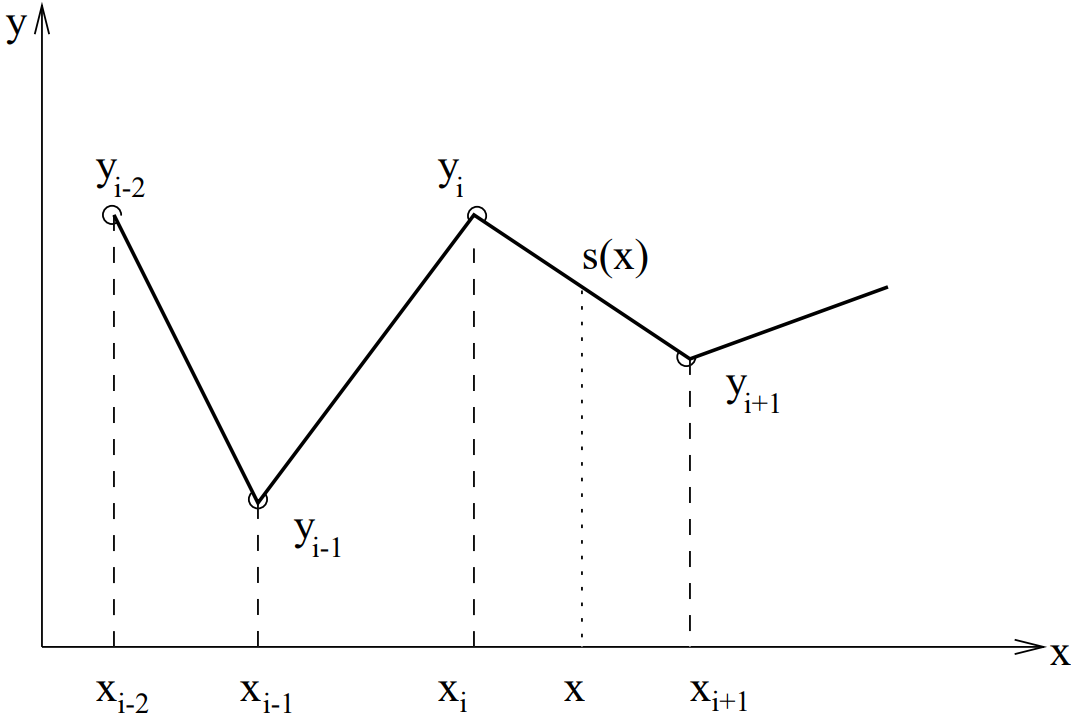
\includegraphics[width=.6\linewidth]{img/4/spline_img_1}
		\end{figure}
		\begin{figure}[h]
			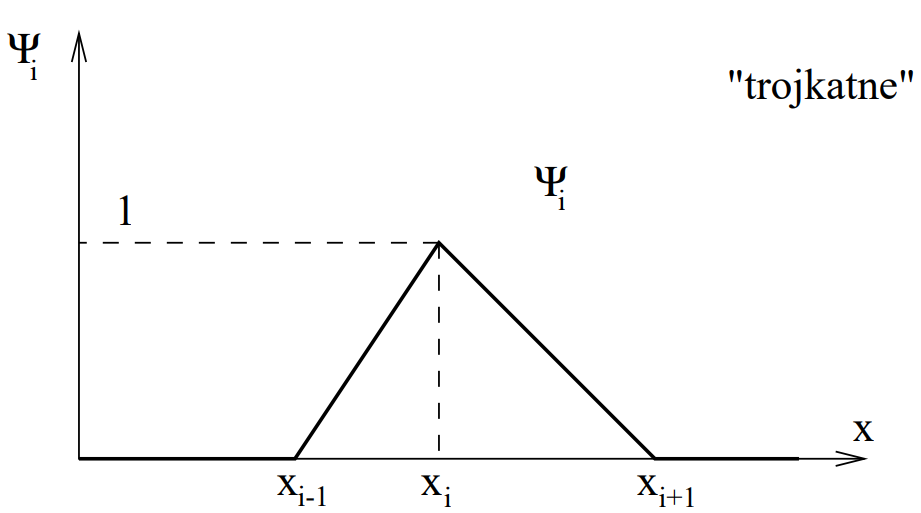
\includegraphics[width=.6\linewidth]{img/4/spline_img_2}
		\end{figure}
    \end{frame}
    
   %%%%%%%%%%%%%%%%%%%%%%%%%%%%%%%5
   \begin{frame}
   		\begin{exampleblock}{}
   			Interpolującą funkcję sklejaną stopnia 1-go można zapisać:
            \[
            	s(x)=\sum_{i=0}^{n}y_{i}\psi_{i}(x)
            \]
            gdzie $\psi_{i}(x), i=0,...,n$ - baza przestrzeni liniowej funkcji sklejanych
            1-go stopnia
   		\end{exampleblock}
        \begin{figure}[h]
			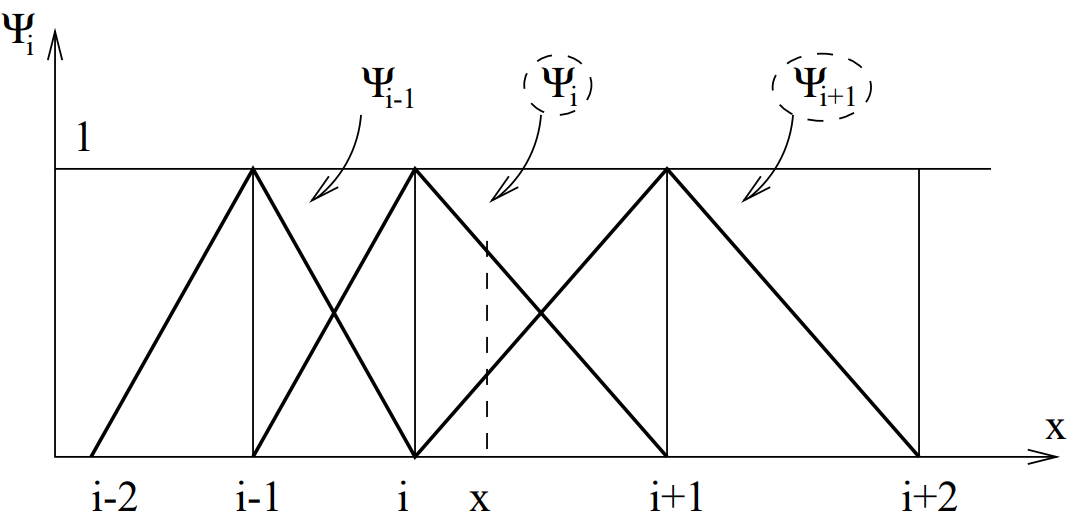
\includegraphics[width=.65\linewidth]{img/4/spline_img_3}
		\end{figure}
   \end{frame}
    
    
    
    
    
    
    
    
    
    
    
    
    
    
    
    
    
    